%%%
%% This is file `sample-sigplan.tex',
%% generated with the docstrip utility.
%%
%% The original source files were:
%%
%% samples.dtx  (with options: `sigplan')
%%
%% IMPORTANT NOTICE:
%%
%% For the copyright see the source file.
%%
%% Any modified versions of this file must be renamed
%% with new filenames distinct from sample-sigplan.tex.
%%
%% For distribution of the original source see the terms
%% for copying and modification in the file samples.dtx.
%%
%% This generated file may be distributed as long as the
%% original source files, as listed above, are part of the
%% same distribution. (The sources need not necessarily be
%% in the same archive or directory.)
%%
%%
%% Commands for TeXCount
%TC:macro \cite [option:text,text]
%TC:macro \citep [option:text,text]
%TC:macro \citet [option:text,text]
%TC:envir table 0 1
%TC:envir table* 0 1
%TC:envir tabular [ignore] word
%TC:envir displaymath 0 word
%TC:envir math 0 word
%TC:envir comment 0 0
%%
%%
%% The first command in your LaTeX source must be the \documentclass command.
%%\documentclass[sigplan,nonacm]{acmart}
\documentclass[sigplan, nonacm]{acmart}\settopmatter{printfolios=true,printccs=false,printacmref=false}

\graphicspath{{pictures/}}
%%
%% \BibTeX command to typeset BibTeX logo in the docs
\AtBeginDocument{%
	\providecommand\BibTeX{{%
			\normalfont B\kern-0.5em{\scshape i\kern-0.25em b}\kern-0.8em\TeX}}}

%% Rights management information.  This information is sent to you
%% when you complete the rights form.  These commands have SAMPLE
%% values in them; it is your responsibility as an author to replace
%% the commands and values with those provided to you when you
%% complete the rights form.
%%\setcopyright{acmcopyright}
\setcopyright{none}
%%\acmJournal{PACMPL}
%%\acmVolume{1}
%%\acmNumber{CONF} % CONF = POPL or ICFP or OOPSLA
%%\acmArticle{1}
%%\acmYear{2021}
%%\acmMonth{9}
%%\acmDOI{}
%%\copyrightyear{2018}
%%\acmYear{2018}
%%\acmDOI{10.1145/1122445.1122456}

%% These commands are for a PROCEEDINGS abstract or paper.
%%\acmConference[Woodstock '18]{Woodstock '18: ACM Symposium%% on Neural
%%  Gaze Detection}{June 03--05, 2018}{Woodstock, NY}
%%\acmBooktitle{Woodstock '18: ACM Symposium on Neural Gaze Detection,
%%  June 03--05, 2018, Woodstock, NY}
%%\acmPrice{15.00}
%%\acmISBN{978-1-4503-XXXX-X/18/06}


%%
%% Submission ID.
%% Use this when submitting an article to a sponsored event. You'll
%% receive a unique submission ID from the organizers
%% of the event, and this ID should be used as the parameter to this command.
%%\acmSubmissionID{123-A56-BU3}

%%
%% The majority of ACM publications use numbered citations and
%% references.  The command \citestyle{authoryear} switches to the
%% "author year" style.
%%
%% If you are preparing content for an event
%% sponsored by ACM SIGGRAPH, you must use the "author year" style of
%% citations and references.
%% Uncommenting
%% the next command will enable that style.
%%\citestyle{acmauthoryear}
\usepackage{xspace}
\usepackage{booktabs}   %% For formal tables:
                        %% http://ctan.org/pkg/booktabs
\usepackage{subcaption} %% For complex figures with subfigures/subcaptions
                        %% http://ctan.org/pkg/subcaption

\usepackage[utf8]{inputenc}
\usepackage[T1]{fontenc}
\usepackage[scaled=0.78]{beramono}
\usepackage{amsmath}
\usepackage{mathtools}
\usepackage{stmaryrd}
%\usepackage{unicode-math}
%\usepackage{MnSymbol}
\usepackage{wasysym}
\usepackage{color}
\usepackage{xcolor,colortbl}
\usepackage{url}
\usepackage{listings}
\usepackage{paralist}
%\usepackage[compact]{titlesec}
\usepackage[font={small}]{caption}
\usepackage{wrapfig}
\usepackage{enumitem}
\usepackage{multicol}
\usepackage{multirow}
\usepackage{makecell}
\usepackage{flushend}
\usepackage{bcprules}
\usepackage{textcomp}
\usepackage{tikz}
\usetikzlibrary{positioning,fit,calc,arrows.meta,arrows,decorations}
\usepackage{pdfpages}
\usepackage{cleveref}
\usetikzlibrary{matrix}
\usepackage{xspace}
\definecolor{light-gray}{gray}{0.85}
\usepackage{stackengine}
\usepackage{mathpartir}
\usepackage{float}
% ----- listings

%\definecolor{ckeyword}{HTML}{7F0055}
\definecolor{ckeyword}{HTML}{000000}
\definecolor{ccomment}{HTML}{3F7F5F}
\definecolor{cstring}{HTML}{2A0099}

\lstdefinelanguage{Scala}%
{morekeywords={
  abstract, sealed, lazy,
  case,catch,char,class,%
  def,do,else,extends,final,finally,for,%
  if,import,implicit,%
  match,module,%
  new,null,undefined,%
  %fun,
  array,
  override,%
  package,private,protected,public,%
  for,public,return,super,%
  this,throw,trait,try,type,%
  val,var,%
  with,while,%
  object,
  let,skip,assert,then,fst,snd,idx,sum,prod,exists,forall,%
  yield,%
  % some scheme keywords
  define, null?, car, cdr
  },%
  sensitive,%
  moredelim=*[il][\bfseries]{\#\#\ },
  morecomment=[l]//,%
  morecomment=[s]{/*}{*/},%
  morestring=[b]",%
  %morestring=[b]',%
  showstringspaces=false%
}[keywords,comments,strings]%

\lstdefinelanguage{Effect}%
{morekeywords={
    effect, yield, return
  },%
  sensitive,%
  moredelim=*[il][\bfseries]{\#\#\ },
  morecomment=[l]//,%
  morecomment=[s]{/*}{*/},%
  morestring=[b]",%
  %morestring=[b]',%
  showstringspaces=false%
}[keywords,comments,strings]%

\lstdefinelanguage{LLVM}%
{morekeywords={
    define, i32, br, icmp, sub, call, mul, phi, ret, label
  },%
  sensitive,%
  moredelim=*[il][\bfseries]{\#\#\ },
  morecomment=[l];,%
  morecomment=[s]{/*}{*/},%
  morestring=[b]",%
  %morestring=[b]',%
  showstringspaces=false%
}[keywords,comments,strings]%

\lstdefinelanguage{CPP}%
{morekeywords={
    using, void, function, if, else, Cont, List
  },%
  sensitive,%
  moredelim=*[il][\bfseries]{\#\#\ },
  morecomment=[l]//,%
  morecomment=[s]{/*}{*/},%
  morestring=[b]",%
  %morestring=[b]',%
  showstringspaces=false%
}[keywords,comments,strings]%


\lstset{
  language=Scala,%
  mathescape=true,%
%  columns=[c]fixed,%
  aboveskip=2pt,%\smallskipamount,
  belowskip=1pt,%\negsmallskipamount,
  lineskip=-1pt,
  basewidth={0.6em, 0.5em},%
%  backgroundcolor=\color{listingbg},
  basicstyle=\ttfamily,
  keywordstyle=\keywordstyle,
  commentstyle=\commentstyle,
  stringstyle=\stringstyle,
%  xleftmargin=0.5cm
  literate={-->}{{$\to$}}2
           {->}{{$\mapsto$}}3
           {<-}{{$\leftarrow$}}2
           {=>}{{$\Rightarrow ~$}}2
           {|-}{{$\ts$}}2
           %{fun}{{$\lambda$}}1
           {idx}{{$\#$}}1
           {array(}{{$\langle.\rangle$(}}3
           {σ}{{$\sigma$}}1
           {ρ}{{$\rho$}}1
           {→}{{$\to$}}1
           {←}{{$\leftarrow$}}1
           {λ}{{$\lambda$}}1
           {α}{{$\alpha$}}1
           {⊔}{{$\sqcup$}}1
           {⊓}{{$\sqcap$}}1
           {⊑}{{$\sqsubseteq$}}1
           {⊤}{{$\top$}}1
           {⊥}{{$\bot$}}1
           {×}{{$\times$}}1
           {τ}{{$\tau$}}1
           {ψ}{{$\psi$}}1
           {Σ}{{$\Sigma$}}1
           {⟨}{{$\langle$}}1
           {⟩}{{$\rangle$}}1
           {π}{{$\pi$}}1
           {∪}{{$\cup$}}2
           %{[[}{{$[\![$}}1
           %{]]}{{$]\!]$}}1
           %{…}{{$\!...$}}1
}

\lstdefinestyle{small}{
  language=Scala,%
  mathescape=true,%
%  columns=[c]fixed,%
  aboveskip=2pt,%\smallskipamount,
  belowskip=1pt,%\negsmallskipamount,
  lineskip=-1pt,
  basewidth={0.6em, 0.45em},%
%  backgroundcolor=\color{listingbg},
  basicstyle=\fontsize{7}{9}\selectfont\ttfamily,
  keywordstyle=\keywordstyle,
  commentstyle=\commentstyle,
  stringstyle=\stringstyle,
%  xleftmargin=0.5cm
  literate={-->}{{$\to$}}3
           {->}{{$\mapsto$}}3
           {=>}{{$\Rightarrow ~$}}2
           {|-}{{$\ts$}}2
           %{fun}{{$\lambda$}}1
           {idx}{{$\#$}}1
           {sum}{{$\Sigma$}}1
           {array(}{{$\langle.\rangle$(}}3
           {σ}{{$\sigma$}}1
           {ρ}{{$\rho$}}1
           {→}{{$\to$}}1
           {λ}{{$\lambda$}}1
           {α}{{$\alpha$}}1
           {⊔}{{$\sqcup$}}1
           {⊓}{{$\sqcap$}}1
           {⊑}{{$\sqsubseteq$}}1
           {⊤}{{$\top$}}1
           {⊥}{{$\bot$}}1
           {×}{{$\times$}}1
           {τ}{{$\tau$}}1
           {ψ}{{$\psi$}}1
           %{[[}{{$[\![$}}1
           %{]]}{{$]\!]$}}1
           %{…}{{$\!...$}}1
}

\lstdefinestyle{extrasmall}{
  language=Scala,%
  mathescape=true,%
%  columns=[c]fixed,%
  aboveskip=2pt,%\smallskipamount,
  belowskip=1pt,%\negsmallskipamount,
  lineskip=-1pt,
  basewidth={0.6em, 0.45em},%
%  backgroundcolor=\color{listingbg},
  basicstyle=\fontsize{6}{8}\selectfont\ttfamily,
  keywordstyle=\keywordstyle,
  commentstyle=\commentstyle,
  stringstyle=\stringstyle,
%  xleftmargin=0.5cm
  literate={-->}{{$\to$}}3
           {->}{{$\mapsto$}}3
           {=>}{{$\Rightarrow ~$}}2
           {|-}{{$\ts$}}2
           %{fun}{{$\lambda$}}1
           {idx}{{$\#$}}1
           {sum}{{$\Sigma$}}1
           {array(}{{$\langle.\rangle$(}}3
           {σ}{{$\sigma$}}1
           {ρ}{{$\rho$}}1
           {→}{{$\to$}}1
           {λ}{{$\lambda$}}1
           {α}{{$\alpha$}}1
           {⊔}{{$\sqcup$}}1
           {⊓}{{$\sqcap$}}1
           {⊑}{{$\sqsubseteq$}}1
           {⊤}{{$\top$}}1
           {⊥}{{$\bot$}}1
           {×}{{$\times$}}1
           %{[[}{{$[\![$}}1
           %{]]}{{$]\!]$}}1
           %{…}{{$\!...$}}1
}

\definecolor{listingbg}{RGB}{240, 240, 240}

\newcommand{\commentstyle}[1]{\color{ccomment}\itshape{#1}}
\newcommand{\keywordstyle}[1]{\color{ckeyword}\bfseries{#1}}
%\newcommand{\keywordstyle}[1]{\color{ckeyword}{#1}}
%\newcommand{\stringstyle}[1]{\color{cstring}\bfseries{#1}}
\newcommand{\stringstyle}[1]{\color{cstring}\text{#1}}

\lstnewenvironment{listing}{\lstset{language=Scala}}{}
\lstnewenvironment{listingtiny}{\lstset{language=Scala,basicstyle=\scriptsize\ttfamily}}{}

\newcommand{\code}[1]{\lstinline[language=Scala,columns=fixed,basicstyle=\ttfamily]|#1|}

% ----- packed items, so we don't waste space
\newenvironment{sitemize}{
\begin{itemize}[leftmargin=2.5ex]
  \setlength{\itemsep}{1pt}
  \setlength{\parskip}{0pt}
  \setlength{\parsep}{0pt}
}{\end{itemize}}

\newenvironment{senumerate}{
\begin{enumerate}[leftmargin=2.5ex]
  \setlength{\itemsep}{1pt}
  \setlength{\parskip}{0pt}
  \setlength{\parsep}{0pt}
}{\end{enumerate}}

\newcommand{\mypar}[1]{{\bf #1.}}

% ----- formal

%\newcommand{\judgement}[2]{{\bf #1} \hfill #2}
%\newcommand{\den}[1]{$\left\llbracket$\;#1\;$\right\rrbracket$}
\newcommand{\den}[1]{\llbracket~#1~\rrbracket}

%\newcommand{\ts}{\,\vdash\,}
\newcommand{\evalsto}{\Downarrow}

\newcommand{\mbind}{\;{\small{\texttt{>>}\hspace{-0.3pt}\raisebox{-0.15pt}{\texttt{=}}}}\;}

%\newcommand{\mbind}{{\small{\texttt{>>}\hspace{-1.7pt}\raisebox{-0.15pt}{\texttt{=}}}}}

\newcommand{\rref}[1]{\textsc{(#1)}}

% ----- comments and todo

\newcommand{\note}[1]{{\color{red}[#1]}}
\newcommand{\snote}[1]{{\color{blue}[#1]}}
\newcommand{\todo}[1]{\note{TODO: #1}}
\newcommand{\rev}[1]{\note{Revision: #1}}

\newcommand{\silent}[1]{}

\newcommand{\hl}[1]{\setlength{\fboxsep}{0pt}\colorbox{light-gray}{#1}}

%\newcommand{\SECFork}{\textsc{sec}$_{\pitchfork}$}
\newcommand{\SECFork}{\textsc{sec}$_{{\mathrlap{<}-}}$}
\newcommand{\SECConc}{\textsc{sec}$_v$}
\newcommand{\SECBack}{\textsc{sec}$_{\hookleftarrow}$}



%%
%% end of the preamble, start of the body of the document source.
\newcommand{\rhyme}{\text{Rhyme}\xspace}
\newcommand{\ul}[1]{\underline{#1}}
\newcommand{\lb}{\{~}
\newcommand{\rb}{~\}}

\newcommand{\Typ}[1]{\ensuremath{\mathsf{#1}}}
\newcommand{\Ast}[1]{\ensuremath{\textsf{\text{#1}}}}
\newcommand{\Def}[1]{\ensuremath{\mathrm{#1}}}
\newcommand{\mit}[1]{\ensuremath{\mathit{#1}}}
\newcommand{\msf}[1]{\ensuremath{\mathsf{#1}}}

\newcommand{\lang}{\textsf{SimpLLVM}\xspace}

\newcommand{\Sem}[3][]{\ensuremath{\llbracket {#2} \rrbracket_{#3}^{#1}}}
\newcommand{\SSem}[2]{\ensuremath{\llbracket {#1} \rrbracket_{#2}^{\#}}}
\newcommand{\State}{\mathbb{S}}
\newcommand{\Address}{\mathcal{A}}
\newcommand{\Mem}{\mathbb{M}}
\newcommand{\Value}{\mathcal{V}}
\newcommand{\Loc}{\msf{Loc}}
\begin{document}
\sloppy

%%
%% The "title" command has an optional parameter,
%% allowing the author to define a "short title" to be used in page headers.
\title{Efficient code generation for loop-free IR}

%%
%% The "author" command and its associated commands are used to define
%% the authors and their affiliations.
%% Of note is the shared affiliation of the first two authors, and the
%% "authornote" and "authornotemark" commands
%% used to denote shared contribution to the research.
\author{Ruiqi Gao}
\email{gao606@purdue.edu}
\affiliation{%
  \institution{Purdue University}
  \city{Lafayette}
  \state{Indiana}
  \country{USA}
  \postcode{47901}
}

\begin{abstract}
  \rhyme is a declarative multi-paradigm query language designed for querying nested data structures like JSON and performing tensor computation. \rhyme performs query optimization and code generation by generating a loop-free, branch-free intermediate representation. \rhyme IR does not explicitly capture program structures; instead, all program structures are implicitly captured by dependencies. This IR design allows for flexible code scheduling and optimization. However, it requires non-trivial reasoning and scheduling of the compiler to generate correct and performant code.\par

  In this paper, we present an efficient code generation algorithm for \rhyme IR. Our algorithm performs aggressive loop scheduling and loop fusion to generate optimized code while ensuring program correctness. It conducts multiple dependency analyses to ensure correctness and uses a heuristic-guided greedy algorithm to perform aggressive loop fusion.
\end{abstract}

\keywords{Loop scheduling, Loop fusion, Code generation}

\maketitle

\section{Introduction}
Rhyme\cite{abeysinghe2024rhyme, abeysingherhyme}, is a declarative language targeting the querying of nested data structures such as JSON and tensors. Rhyme draws inspiration from existing query languages like JQ \cite{jq}, GraphQL \cite{graphql}, and XQuery \cite{xquery} for querying nested data structures. Similar to Datalog \cite{datalog} and JSONPath \cite{jsonpath}, Rhyme employs logic variables * to explicitly represent iterators over data sources. Inspired by functional languages like Verse \cite{verse} and Curry \cite{curry}, Rhyme uses unification to represent aggregation. Additionally, Rhyme can express tensor computations mathematically, akin to Einstein notation \cite{einops, einsumblog, tensor_comprehensions}.

Rhyme supports the expression of both traditional data processing operations such as aggregation, joins, and group-by, and mathematical computations like matrix multiplication and transpose in a unified language. Rhyme also includes internal support for data visualization, allowing users to perform various workloads in a single language without relying on multiple backends.

To perform query optimization and code generation, Rhyme generates an intermediate representation (IR). Traditional IRs like LLVM \cite{lattner2004llvm} statically represent the program structure within the IR itself, with all statements scoped within blocks. Therefore, any code motion, such as hoisting, requires dependency analysis to ensure correctness. In contrast, the Sea of Nodes IR \cite{hotspot} does not explicitly impose program structure; instead, it captures all program structures implicitly through dependencies. This design allows for flexible code motion and local optimizations, with the program structure reconstructed during code generation. Inspired by \cite{rompf2010lightweight} and \cite{bravcevac2023graph}, Rhyme generates a loop-free, branch-free IR, capturing program structures via both data and control dependencies. While this design simplifies optimizations like loop hoisting and code scheduling, it complicates code generation, as the program structure must be reconstructed. The code generator needs to determine the order between loops, figure out how loops should be nested, and place instructions inside loops. Careless code placement, such as inserting an instruction inside a deeper loop nest, will cause redundant computations. This may also lead to incorrect results if the instruction corresponds to an aggregation in the source language. Therefore, the code generator must produce efficient code while respecting the semantics of the source language.\par

In this paper, we introduce a novel code generation algorithm for Rhyme IR. It performs intelligent loop scheduling to derive an efficient loop structure for the program and utilizes a heuristic-guided algorithm to perform aggressive loop fusion. This optimization reduces extra loop control overhead, enables more optimization opportunities for the backend compiler, and reduces memory usage. The code generator guarantees program correctness by precomputing several program dependencies while respecting the semantic constraints of aggregations.
\subsection{Paper Structure}
\iffalse
The paper is organized as follows: \par \par
In section \ref{rhymeir}, we will look at the structure of Rhyme IR and its operators. This severs as a background for our code generation algorithm\par
In section \ref{buildeps}, we will present several constraints that our code generator must follow to ensure program correctness. Then we will present the dependencies we need to pre-compute, these dependencies will be followed by the code generator during code scheduling to guarantee correctness.\par
In section \ref{codeschedule}, we will dive deep into our code scheduling algorithm. We will investigate how the loop are scheduled and fused to improve performance. We will also look at the heuristic used to perform greedy scheduling.\par
In section \ref{evaluation}, we compare the performance of old and new code generator of Rhyme, compare the generated code and explain the differences.\par
In section \ref{conclusion}, we summarize the work and draw some conclusions.
\fi
The paper is organized as follows:\par \par
In Section \ref{rhymeir}, we explore the structure of Rhyme IR and its operators, providing essential background for our code generation algorithm.\par
In Section \ref{buildeps}, we present several constraints that our code generator must adhere to in order to ensure program correctness. We then detail the dependencies that need to be pre-computed, guiding the code generator during code scheduling to guarantee correctness.\par
In Section \ref{codeschedule}, we delve into our code scheduling algorithm, examining how loops are scheduled and fused to improve performance. We also discuss the heuristic employed for greedy scheduling.\par
In Section \ref{evaluation}, we compare the old and new code generators of Rhyme, compare the generated code and explain the differences.\par
Finally, in Section \ref{conclusion}, we summarize our findings and draw conclusions.

\section{Rhyme IR}\label{rhymeir}
\iffalse
Rhyme IR consists of two types of operators: \textit{generators} and \textit{assignments}:\begin{itemize}
  \item Generators are operators responsible for iterating over data sources and intermediate results. Generator operations are transformed into loops in the generated code. User can use \inline{*} to represent a generator. For example, \inline{data.*} binds the generator \inline{*} to \inline{data}, it will iterate over \inline{data}, enumerating its values.
  \item Assignments are operators that model all the computation for intermediate or final results. Rhyme generates temporaries in the IR to store intermediate results for sub-queries. For example, in query \inline{sum(data.*A.val) + sum(data.*B.val)}, \inline{sum(data.*A.val)} and \inline{sum(data.*B.val)} are stored in two temporaries - \inline{tmp[1]} and \inline{tmp[2]}. The final result is stored in \inline{tmp[0]}, and an assignment \inline{tmp[0] = tmp[1] + tmp[2]} is generated to compute the addition of the two sum.
\end{itemize}
As we mentioned above, intermediate results are stored in temporaries. Generators can iterate over temporaries, this will introduce a generator to temp dependencies. Also, since assignments can use temporaries as operand and write the result to temporaries, this create an assignment to temp dependencies. An assignment's right hand side (its operands) may also indexing into a data source/intermediate result by a generator. This gives us assignment to generator dependencies.\par
Each assignment will write to a temporaries, i.e., its writeSym. There maybe multiple assignments write to a same temp. To ensure the correct ordering of those assignments and guarantee program correctness, Rhyme assigns write ranks to assignments that write to the same temp during IR generation. All assignments to the same temp must be ordered by their write rank. This gives us assignment to assignment dependencies. Since there maybe multiple assignments write to a temp, the temporary variable is not fully materialized until the last assignment that write to it. This introduces temp to assignment dependencies.\par
Our brief discussions above already illustrate that the Rhyme IR models the complicated dependencies between generator, assignment and temp variables. When we generate code, we must faithful follow these dependencies in the IR to ensure program correctness.\par
Besides the dependencies mentioned above, we also need to consider the semantic of aggregations in the IR. For temporaries that store aggregation results, we need to wait for it to be fully materialized in order to use it, otherwise we may use a partial aggregation and gives incorrect results. This will add extra dependencies in the IR level, we will talk more in detail about this in Section \ref{buildeps}.
\fi
Rhyme IR consists of two types of operators: \textit{generators} and \textit{assignments}:\begin{itemize}
  \item Generators are operators responsible for iterating over data sources and intermediate results. Generator operations are transformed into loops in the generated code. Users can use \inline{*} to represent a generator. For example, \inline{data.*} binds the generator \inline{*} to \inline{data}, iterating over \inline{data} and enumerating its values.

  \item Assignments are operators that model all computations for intermediate or final results. Rhyme generates temporaries in the IR to store intermediate results for sub-queries. For instance, in the query \inline{sum(data.*A.val) + sum(data.*B.val)}, \inline{sum(data.*A.val)} and \inline{sum(data.*B.val)} are stored in two temporaries - \inline{tmp[1]} and \inline{tmp[2]}. The final result is stored in \inline{tmp[0]}, and an assignment \inline{tmp[0] = tmp[1] + tmp[2]} is generated to compute the addition of the two sums.
\end{itemize}
As mentioned above, intermediate results are stored in temporaries. Generators can iterate over temporaries, introducing a generator-to-temp dependency. Additionally, since assignments can use temporaries as operands and write the result to temporaries, this creates an assignment-to-temp dependency. An assignment's right-hand side (its operands) may also index into a data source/intermediate result by a generator, resulting in assignment-to-generator dependencies.\par

Each assignment will write to a temporary, i.e., its writeSym. There may be multiple assignments writing to the same temp. To ensure the correct ordering of those assignments and guarantee program correctness, Rhyme assigns write ranks to assignments that write to the same temp during IR generation. All assignments to the same temp must be ordered by their write rank. This results in assignment-to-assignment dependencies. Since there may be multiple assignments writing to a temp, the temporary variable is not fully materialized until the last assignment that writes to it. This introduces temp-to-assignment dependencies.\par

Our brief discussions above illustrate that the Rhyme IR models the complex dependencies between generators, assignments, and temp variables. When generating code, we must faithfully follow these dependencies in the IR to ensure program correctness.\par

In addition to the dependencies mentioned above, we also need to consider the semantics of aggregations in the IR. For temporaries that store aggregation results, we need to wait for them to be fully materialized before using them; otherwise, we may use a partial aggregation and obtain incorrect results. This introduces additional dependencies at the IR level, which we will discuss in more detail in Section \ref{buildeps}.
\section{Semantic constraints and Dependency construction}\label{buildeps}
\iffalse
The code generator needs to follow several semantic constraints to ensure program correctness and generate efficient code. The code generator also needs to respect the dependencies between assignments and generators in th IR during code scheduling. In this section, we will delve into this two part. This will give us a deeper understanding of the intuition of our code scheduling algorithm. Since generators will be transformed into loops and assignments will be transformed into statements in the generated code. \par\textbf{Note: From now on, generator/loop and assignment/statement will be used interchangeably.}
\subsection[]{Semantic constraints}
We want to list several semantic constraints for the code generators here. These constraints will discipline the code generation for assignments and generators:
\begin{enumerate}
  \item \textbf{a statement will be only emitted once.} Since assignment model computations for intermediate and final results, they can be only emitted once.
  \item \textbf{a loop maybe generated multiple times.} There could multiple assignments depend on one generator. The code generator can choose to either schedule them in one loop body or distribute them among multiple loops that correspond to the same generator. If a generator have n assignments depend on it. It can be generated at most n times.
  \item \textbf{a statement will be emitted inside and only inside the loops it depends on.} This means we will never emit a statement inside irrelevant loops. Emitting an assignment inside irrelevant loops not only introduces extra overhead but may also gives incorrect results if the assignment computes an aggregation.
  \item \textbf{statements and loops will be emitted while faithfully following the dependencies between them.} When emit statements and loops, the code generator must follow the dependencies between them to ensure program correctness. We will talk about this more in detail in subsection \ref{depsonstruct}.
\end{enumerate}
These four semantic constraints lay the foundation for our code generator. Any code generation algorithm following these constraints can guarantee the correctness of their generated program. A smart code generator, on the other hand, need to fuse different statements' loops together as much as possible to improve performance.
\fi
The code generator needs to follow several semantic constraints to ensure program correctness and generate efficient code. The code generator also needs to respect the dependencies between assignments and generators in the IR during code scheduling. In this section, we will delve into these two parts. This will give us a deeper understanding of the intuition behind our code scheduling algorithm. Since generators will be transformed into loops and assignments will be transformed into statements in the generated code.\par

\textbf{Note: From now on, generator/loop and assignment/statement will be used interchangeably.}

\subsection[]{Semantic constraints}\label{semconst}

We want to list several semantic constraints for the code generator here. These constraints will discipline the code generation for assignments and generators:

\begin{enumerate}
\item \textbf{A statement will only be emitted once.} Since assignments model computations for intermediate and final results, they can only be emitted once.
\item \textbf{A loop may be generated multiple times.} There could be multiple assignments depending on one generator. The code generator can choose to either schedule them in one loop body or distribute them among multiple loops that correspond to the same generator. If a generator has n assignments depending on it, it can be generated at most n times.
\item \textbf{A statement will be emitted inside and only inside the loops it depends on.} This means we will never emit a statement inside irrelevant loops. Emitting an assignment inside irrelevant loops not only introduces extra overhead but may also give incorrect results if the assignment computes an aggregation.
\item \textbf{Statements and loops will be emitted while faithfully following the dependencies between them.} When emitting statements and loops, the code generator must follow the dependencies between them to ensure program correctness. We will talk about this in more detail in subsection \ref{depsonstruct}.
\end{enumerate}

These four semantic constraints lay the foundation for our code generator. Any code generation algorithm following these constraints can guarantee the correctness of its generated program. However, these constraints do not enforce a strict program structure. Statements that are independent of each other can be scheduled in an arbitrary order. A generator can be emitted multiple times, so statements can be placed among them as long as the dependencies are followed. Therefore, a smart code generator needs to fuse different statements' loops together as much as possible to improve performance.
\subsection[]{Dependency construction}\label{depsonstruct}
\iffalse
We briefly explored the dependencies of Rhyme IR in Section \ref{rhymeir}. We already observed a complicated dependency between assignments, generators and temporaries. Dependency to a temp can be inlined to the last assignment that update it. Therefore, we obtain four kinds of dependencies:
\begin{enumerate}
  \item \textbf{assignment-to-assignment} dependencies. These dependencies are introduced by the def-use effect of assignments. If assignment a uses temp1, and the last assignment that modifies temp1 is b, then a depends on b. Also, an assignment depends on the previous assignment that update the same temp (based on the write rank).
  \item \textbf{assignment-to-generator} dependencies. If an assignment uses a generator (the rhs indexing into a temp by a generator or the lhs is grouped by the generator), the assignment depends on the generator.
  \item \textbf{generator-to-assignment} dependencies. If a generator iterates over a temp, it depends on the last assignment that modifies this temp.
  \item \textbf{generator-to-generator} dependencies. If the value that generator A iterates over is generated by another generator B, A depends on B. For example, in query \inline{data.*A.*B}, \inline{*A} depends on \inline{*B}.
\end{enumerate}
Dependencies are inherently transitive, if A depends on B and B depends on C, A also depends on C. According to our semantic constraints, assignment are only emitted once. Therefore, we use assignment/statement as the basic unit of dependencies. \par During dependencies construction phase, we first pre compute two types of dependencies:
\begin{itemize}
  \item \textbf{stmtdeps}: For each assignment/statement, this tracks all the assignments it transitively depends on, deriving from all four type of dependencies listed above.
  \item \textbf{loopdeps}: For each assignment/statement, this tracks all the generators/loops it transitively depends on, i.e., the loop nests it resides in. When tracking loopdeps, we only follow assignment-to-generator and generator-to-generator dependencies. We never track loop dependencies beyond  assignments. The reason for it is simple: if assignment s1 depends on loop l1, and l1 depends on assignment s2. l1 only depends on the materialized result that s2 writes to. If s2 again depends on l2, the result is not fully materialized until l2 closes, therefore l1 does not need to be nested inside l2. As a result, s1 also does not depend on l2.
\end{itemize}
stmtdeps stores the dependencies between assignments, so we need to emit assignments following the topological order of this dependencies graph. For an assignment, when all prerequisites in stmtdeps are emitted, the assignment is ready to be emitted, although it may not have all loops opened at the moment. \par loopdeps then tells us the loops that an assignment need to be emitted in. An assignment can only be emitted when all loops it depends on are opened and all its prerequisites in stmtdeps are emitted.\par
\fi
We briefly explored the dependencies of Rhyme IR in Section \ref{rhymeir}. We already observed a complicated dependency between assignments, generators, and temporaries. Dependency to a temp can be inlined to the last assignment that updates it. Therefore, we obtain four kinds of dependencies:

\begin{enumerate}
\item \textbf{Assignment-to-assignment} dependencies: These dependencies are introduced by the def-use effect of assignments. If assignment $a$ uses $temp1$, and the last assignment that modifies $temp1$ is $b$, then $a$ depends on $b$. Also, an assignment depends on the previous assignment that updates the same temp (based on the write rank).
\item \textbf{Assignment-to-generator} dependencies: If an assignment uses a generator (the rhs indexing into a temp by a generator or the lhs is grouped by the generator), the assignment depends on the generator.
\item \textbf{Generator-to-assignment} dependencies: If a generator iterates over a temp, it depends on the last assignment that modifies this temp.
\item \textbf{Generator-to-generator} dependencies: If the value that generator $A$ iterates over is generated by another generator $B$, $A$ depends on $B$. For example, in query \inline{data.*A.*B}, \inline{*B} depends on \inline{*A}.
\end{enumerate}

Dependencies are inherently transitive: if $A$ depends on $B$ and $B$ depends on $C$, $A$ also depends on $C$. According to our semantic constraints, assignments are only emitted once. Therefore, we use assignment/statement as the basic unit of dependencies.\par

During the dependencies construction phase, we first pre-compute two types of dependencies:

\begin{itemize}
\item \textbf{Stmtdeps}: For each assignment/statement, this tracks all the assignments it transitively depends on, derived from all four types of dependencies listed above.
\item \textbf{Loopdeps}: For each assignment/statement, this tracks all the generators/loops it transitively depends on, i.e., the loop nests it resides in. When tracking loopdeps, we only follow assignment-to-generator and generator-to-generator dependencies. We never track loop dependencies beyond assignments. The reason for this is simple: if assignment $s1$ depends on loop $l1$, and $l1$ depends on assignment $s2$, $l1$ only depends on the materialized result that $s2$ writes to. If $s2$ again depends on $l2$, the result is not fully materialized until $l2$ closes, therefore $l1$ does not need to be nested inside $l2$. As a result, $s1$ also does not depend on $l2$.
\end{itemize}

Stmtdeps stores the dependencies between assignments, so we need to emit assignments following the topological order of this dependency graph. For an assignment, when all prerequisites of it in stmtdeps are emitted, the assignment is ready to be emitted, although it may not have all loops opened at the moment.\par

Loopdeps then tell us the loops that an assignment needs to be emitted in. An assignment can only be emitted when all loops it depends on are opened and all its prerequisites in stmtdeps are emitted.\par

\iffalse
Although stmtdeps and loopdeps already give us a lot of information about the program, it still does not fully model all the required dependencies. Rhyme is a query language by design, therefore it supports different types of aggregations - sum, count, min, max, etc. If an assignment computes the result of an aggregation and stores the result in a temp. The aggregation is only fully materialized until all the loops it depends on are all closed, i.e., the aggregation is fully computed. Any assignment that uses this temp will need to wait for the aggregation to be fully materialized, otherwise it may uses a partial aggregation and produce incorrect results.\par
This observation inspires two extra dependencies we need to track to ensure program correctness:
\begin{itemize}
  \item \textbf{stmt2stmtByLoop}: if statement s1 depends on s2, this tracks the loops of s2 that need to be closed for s1 to be emittable. This is needed for aggregation statements. We need to wait for all dependent loops to close for the aggregation to be fully materialized.
  \item \textbf{stmt2stmtloopAfterloop}: if assignment s1 depends on s2, this tracks the pair of loops (l1, l2) such that: s1 depends on l1, s2 depends on l2 and s1's l1 needed to be emitted after s2's l2. This gives an ordering of loops and will be used in the heuristic for loop scheduling.
\end{itemize}
We currently only track stmt2stmtByLoop and stmt2stmtloopAfterloop between statements that write to different temporary variables. If s1 depends on s2, we compute these two dependencies as follows:\par
If s2 depends on loop l and s1 does not. Then s1 need to wait for s2's l loop to close so that the temp s2 writes to is fully materialized. So we need to set \inline{stmt2stmtByLoop[s1][s2][l] = true}. If s1 depends on l, s1 may or may not need to wait for s2's l to close, depending on the computation s2 models and how s1 uses s2's result. For example, if s2 writes to \inline{temp1[*l]} and s1 uses \inline{temp1[*l]}, s1 and s2 can be put in the same loop body for l. However, we can perform arithmetic operations on the generators in Rhyme. Since generator represents iterator, we can offset the generator for indexing. So, if s2 writes to \inline{temp1[*l]} and s1 uses \inline{temp1[func(*l)]}, s1 may need to wait for \inline{temp1} to be fully materialized to use it. Therefore, s1 and s2 may or may not be able to be put in the same l loop, depending on the semantic of \inline{func}. With more precise dependency analysis and reasoning, we can relax the requirements for stmt2stmtByLoop and explore more optimization opportunities. stmt2stmtByLoop offers a precise, fine-grained dependencies between statements with regard to loops. It gives the compiler more information about how loops should be scheduled. And the compiler construct stmt2stmtByLoop to reflect the semantic of different assignments and the dependencies between them.
\fi
Although \texttt{stmtdeps} and \texttt{loopdeps} already provide a lot of information about the program, they still do not fully model all the required dependencies. Rhyme is a query language by design; therefore, it supports different types of aggregations - sum, count, min, max, etc. If an assignment computes the result of an aggregation and stores the result in a temporary variable, the aggregation is only fully materialized when all the loops it depends on are closed, i.e., the aggregation is fully computed. Any assignment that uses this temporary variable will need to wait for the aggregation to be fully materialized; otherwise, it may use a partial aggregation and produce incorrect results.\par
This observation inspires two extra dependencies we need to track to ensure program correctness:
\begin{itemize}
\item \textbf{stmt2stmtByLoop}: if statement \texttt{s1} depends on \texttt{s2}, this tracks the loops of \texttt{s2} that need to be closed for \texttt{s1} to be emittable. This is needed for aggregation statements. We need to wait for all dependent loops to close for the aggregation to be fully materialized.
\item \textbf{stmt2stmtloopAfterloop}: if assignment \texttt{s1} depends on \texttt{s2}, this tracks the pair of loops (\texttt{l1}, \texttt{l2}) such that: \texttt{s1} depends on \texttt{l1}, \texttt{s2} depends on \texttt{l2} and \texttt{s1}'s \texttt{l1} needs to be emitted after \texttt{s2}'s \texttt{l2}. This gives an ordering of loops and will be used in the heuristic for loop scheduling.
\end{itemize}
We currently only track \texttt{stmt2stmtByLoop} and \texttt{stmt2stmtloopAfterloop} between statements that write to different temporary variables. If \texttt{s1} depends on \texttt{s2}, we compute these two dependencies as follows:\par
If \texttt{s2} depends on loop \texttt{l} and \texttt{s1} does not, then \texttt{s1} needs to wait for \texttt{s2}'s \texttt{l} loop to close so that the temporary variable \texttt{s2} writes to is fully materialized. So we need to set \inline{stmt2stmtByLoop[s1][s2][l] = true}. If \texttt{s1} depends on \texttt{l}, \texttt{s1} may or may not need to wait for \texttt{s2}'s \texttt{l} to close, depending on the computation \texttt{s2} models and how \texttt{s1} uses \texttt{s2}'s result. For example, if \texttt{s2} writes to \texttt{temp1[*l]} and \texttt{s1} uses \texttt{temp1[*l]}, \texttt{s1} and \texttt{s2} can be put in the same loop body for \texttt{l}. However, we can perform arithmetic operations on the generators in Rhyme. Since a generator represents an iterator, we can offset the generator for indexing. So, if \texttt{s2} writes to \texttt{temp1[*l]} and \texttt{s1} uses \texttt{temp1[func(*l)]}, \texttt{s1} may need to wait for \texttt{temp1} to be fully materialized to use it. Therefore, \texttt{s1} and \texttt{s2} may or may not be able to be put in the same \texttt{l} loop, depending on the semantics of \texttt{func}. With more precise dependency analysis and reasoning, we can relax the requirements for \texttt{stmt2stmtByLoop} and explore more optimization opportunities. \texttt{stmt2stmtByLoop} offers precise, fine-grained dependencies between statements with regard to loops. It gives the compiler more information about how loops should be scheduled. And the compiler constructs \texttt{stmt2stmtByLoop} to reflect the semantics of different assignments and the dependencies between them.\par
\iffalse
stmt2stmtloopAfterloop, on the other hand, is derived from stmt2stmtByLoop. And it is constructed to hint an ordering of loops. If \inline{stmt2stmtByLoop[s1][s2][l2] = true}, we know that s1 need to wait for s2'l2 loop to close. This means s1 needs to be emitted after s2's l2 loop closes. If s1 depends on l1 and s2 does not depend on l1. s1's l1 loop needs to be scheduled after s2's l2 loop, and we set \inline{stmt2stmtloopAfterloop[s1][s2][l1][l2] = true}. We never emit a statement inside irrelevant loops according to the semantic constraints described in subsection \ref{semconst}.Since s1 does not depend on l2 and s2 does not depend on l1. We will never emit s1 inside l2 and emit s2 inside l1, s1's l1 and s2's l2 can not be nested within each other. Since we need to emit s1 after s2's l2, s1'l1 must also be scheduled after s2's l2. This enforecs an ordering between l1 and l2 per s1 and s2. Whenever we have a list of statements that are ready to be issued, we can merge all the per statement pair loop order among these statements into a local loopAfterLoop relation. This local loopAfterLoop relation tells us the order by which we should emit loops. This will be used as a hint for loop scheduling, which we will talk more in detail in Section \ref{codeschedule}.
\fi
\texttt{stmt2stmtloopAfterloop}, on the other hand, is derived from \texttt{stmt2stmtByLoop}, and it is constructed to hint an ordering of loops. If \inline{stmt2stmtByLoop[s1][s2][l2] = true}, we know that \texttt{s1} needs to wait for \texttt{s2}'s \texttt{l2} loop to close. This means \texttt{s1} needs to be emitted after \texttt{s2}'s \texttt{l2} loop closes. If \texttt{s1} depends on \texttt{l1} and \texttt{s2} does not depend on \texttt{l1}, \texttt{s1}'s \texttt{l1} loop needs to be scheduled after \texttt{s2}'s \texttt{l2} loop, and we set \inline{stmt2stmtloopAfterloop[s1][s2][l1][l2] = true}. We never emit a statement inside irrelevant loops according to the semantic constraints described in subsection \ref{semconst}. Since \texttt{s1} does not depend on \texttt{l2} and \texttt{s2} does not depend on \texttt{l1}, we will never emit \texttt{s1} inside \texttt{l2} and emit \texttt{s2} inside \texttt{l1}. \texttt{s1}'s \texttt{l1} and \texttt{s2}'s \texttt{l2} can not be nested within each other. Since we need to emit \texttt{s1} after \texttt{s2}'s \texttt{l2}, \texttt{s1}'s \texttt{l1} must also be scheduled after \texttt{s2}'s \texttt{l2}. This enforces an ordering between \texttt{l1} and \texttt{l2} per \texttt{s1} and \texttt{s2}. Whenever we have a list of statements that are ready to be issued, we can merge all the per statement-pair loop order among these statements into a local \texttt{loopAfterLoop} relation. This local \texttt{loopAfterLoop} relation tells us the order by which we should emit loops. This will be used as a hint for loop scheduling, which we will talk about in more detail in Section \ref{codeschedule}.\par
In this section, we delve deep into the semantic constraints and dependency construction of our code generator. The constraints and dependencies form the basis of our code generation algorithm to ensure correctness. We will discuss the loop scheduling algorithm in more detail in the next section.
\section{Code scheduling}\label{codeschedule}
\iffalse
Semantic constraints and pre-computed dependencies discipline code generation, enforcing restrictions on the code generator to guarantee correctness. They decide which statements should be scheduled before a statement. They restrict which loops a statement need to reside in. They also decide what loops need to be closed for a statement to be issuable.  However, they do not restrict a program structure. And they leave the code generator a lot of freedom to schedule statements and loops. \par
As we mentioned in subsection \ref{semconst}, a loop can be emitted multiple times. Although we want to put all statements that depend on a generator in one loop body, sometimes it is infeasible due to the aforementioned \texttt{stmt2stmtByLoop} and \texttt{stmt2stmtloopAfterloop} dependencies. For example, consider the following IR snippet:
\begin{lstlisting}[numbers=left]
  tmp[1] += data1[*A]['val1']
  tmp[2] += (data2[*B]['val2'] / tmp[1])
  tmp[3][*A] = data1[*A]['val3'] / tmp[2]
  \end{lstlisting}
The semantic meaning of this snippet is not irrelevant here, we only care about the dependencies captured in the IR. Assignment 1 uses *A in the rhs, so it depends on *A, same thing for assignment 3, and assignment 2 depends on *B. Assignment 3 depends on assignment 2, and assignment 2 depends on assignment 1 due to the def-use chain. Since both assignment 1 and 2 compute an aggregation (sum), their loop (*A and *B) need to be closed for tmp[1] and tmp[2] to be fully materialized. Therefore assignment 2 need to wait for assignment 1's *A loop to close, assignment 3 need to wait for assignment 2's *B loop to close.\par
Ideally, we want to put both assignment 1 and 3 in the same *A loop to reduce the loop control overhead, i.e., fuse assignment 1 and 3's *A loop. However, this is not possible due to the extra dependency of assignment 2. Assignment 2 needs to be emitted after assignment 1. So assignment 2's *B loop should be emitted after assignment 1's *A loop closes. Similarly, assignment 3's *A loop need to be after assignment 2's *B loop. So assignment 3's *A loop can only be scheduled after assignment1's *A loop closes. This prevents assignment 1 and 3 from being placed in the same *A loop.\par
For large and complex applications, there are multiple fusion opportunities when scheduling code. And the compiler must carefully schedule loops to maximize fusion. For example, consider the following IR snippet:
\begin{lstlisting}[numbers=left]
  tmp[1][*A] += data1[*A][*B]['val1']
  tmp[2][*A] = tmp[1][*A] + data2[*A]['val2']
  tmp[3][*A] = tmp[1][*A] + data3[*A]['val3']
  \end{lstlisting}
Assignment 1 resides in both *A and *B loops, assignment 2 and 3 only resides in *A loop. Also, assignment 2 and 3 need to be scheduled after assignment 1 due to dependencies. We we emit assignment 1, if we choose to first emit *B loop and then emit *A loop inside *B loop. We can not put the succeeding assignments inside the nested *A loop as these assignments are only dependent on the *A loop, so they can not be nested within *B. Therefore, the compiler needs to close the *B and *A loop nest. Then reopen *A loop to emit assignment 2 and 3. If we choose to emit *A loop first when emitting assignment 1, this redundance will be eliminated and we can fuse assignment 1,2,3's *A loop.\par
As we observed before, the code generator need to perform non-trivial reasoning to generate optimal loop structure for the IR while satisfy the dependencies. The goal is to maximize loop fusion to improve performance. We now present our heuristic-guided loop scheduling algorithm that can perform aggressive loop fusion efficiently.\par
\fi
Semantic constraints and pre-computed dependencies discipline code generation, enforcing restrictions on the code generator to guarantee correctness. They determine which statements should be scheduled before others, restrict the loops in which a statement can reside, and dictate which loops need to be closed for a statement to be issuable. However, they do not restrict the program structure, leaving the code generator with considerable freedom to schedule statements and loops.

As mentioned in subsection \ref{semconst}, a loop can be emitted multiple times. Although we aim to place all statements that depend on a generator in one loop body, sometimes it is infeasible due to the aforementioned \texttt{stmt2stmtByLoop} and \texttt{stmt2stmtloopAfterloop} dependencies. For example, consider the following IR snippet:
\begin{lstlisting}[numbers=left]
tmp[1] += data1[*A]['val1']
tmp[2] += (data2[*B]['val2'] / tmp[1])
tmp[3][*A] = data1[*A]['val3'] / tmp[2]
\end{lstlisting}
The semantic meaning of this snippet is not relevant here; we only care about the dependencies captured in the IR. Assignment 1 uses \texttt{*A} in the right-hand side (RHS), so it depends on \texttt{*A}; the same goes for assignment 3, and assignment 2 depends on \texttt{*B}. Assignment 3 depends on assignment 2, and assignment 2 depends on assignment 1 due to the def-use chain. Since both assignment 1 and 2 compute an aggregation (sum), their loops (\texttt{*A} and \texttt{*B}) need to be closed for \texttt{tmp[1]} and \texttt{tmp[2]} to be fully materialized. Therefore, assignment 2 needs to wait for assignment 1's \texttt{*A} loop to close, and assignment 3 needs to wait for assignment 2's \texttt{*B} loop to close.

Ideally, we want to put both assignment 1 and 3 in the same \texttt{*A} loop to reduce the loop control overhead, i.e., fuse assignment 1 and 3's \texttt{*A} loop. However, this is not possible due to the extra dependency of assignment 2. Assignment 2 needs to be emitted after assignment 1. So assignment 2's \texttt{*B} loop should be emitted after assignment 1's \texttt{*A} loop closes. Similarly, assignment 3's \texttt{*A} loop needs to be after assignment 2's \texttt{*B} loop. Thus, assignment 3's \texttt{*A} loop can only be scheduled after assignment 1's \texttt{*A} loop closes, preventing assignment 1 and 3 from being placed in the same \texttt{*A} loop.

For large and complex applications, there are multiple fusion opportunities when scheduling code. The compiler must carefully schedule loops to maximize fusion. For example, consider the following IR snippet:\par
\begin{figure}[H]
\begin{lstlisting}[numbers=left]
tmp[1][*A] += (data0[*A]['val0'] + data1[*B]['val1'])
tmp[2][*A] = tmp[1][*A] + data2[*A]['val2']
tmp[3][*A] = tmp[1][*A] + data3[*A]['val3']
\end{lstlisting}
\caption{}
\label{loopheu}
\end{figure}
Assignment 1 resides in both \texttt{*A} and \texttt{*B} loops, while assignment 2 and 3 only reside in the \texttt{*A} loop. Also, assignment 2 and 3 need to be scheduled after assignment 1 due to dependencies. When we emit assignment 1, if we first emit the \texttt{*B} loop and then the \texttt{*A} loop inside the \texttt{*B} loop, we cannot put the succeeding assignments inside the nested \texttt{*A} loop as these assignments are only dependent on the \texttt{*A} loop, so they cannot be nested within \texttt{*B}. Therefore, the compiler needs to close the \texttt{*B} and \texttt{*A} loop nest and then reopen the \texttt{*A} loop to emit assignment 2 and 3. If we choose to emit the \texttt{*A} loop first when emitting assignment 1, this redundancy will be eliminated, and we can fuse assignment 1, 2, and 3's \texttt{*A} loop.

As observed before, the code generator needs to perform non-trivial reasoning to generate an optimal loop structure for the IR while satisfying the dependencies. The goal is to maximize loop fusion to improve performance. We now present our heuristic-guided loop scheduling algorithm, which can perform aggressive loop fusion efficiently.
\subsection*{Loop scheduling algorithm}
\iffalse
We use a heuristic guided approach to perform efficient loop scheduling. As we mentioned before, we use statement as the basic unit for code scheduling. \par
\paragraph*{Iteratively emitting statements} If all prerequisite statements of a statement are emitted and have their loops (with respect to stmt2stmtByLoop) closed, we call this statement \textbf{ready}. If all dependent loops of a statement are opened, we call this statement \textbf{inloops}. If a statement is both ready and inloops, we call this statement \textbf{emittable}, and we can emit the statement. Since we have pre computed both stmtdeps, loopdeps and stmt2stmtByLoop, the first stage is trivial. We check for all remaining statements whether they are emittable, and emit them if so. We will iteratively emit statements until there are no emittable statements left.\par
Although there are no emittable statements, some statements may still be ready, they just do not have all their dependent loops opened. If there are no ready statements, this means some statement are waiting for its prerequisites' loops to close. Then we close the current loop and return to the parent loop scope.\par
 If there are several ready statements and they depend on multiple loops, we need to choose which loop to open next carefully. Careless choice of which loop to open next may eliminate future opportunities for loop fusion and generate suboptimal code. We also may take stmt2stmtloopAfterloop in to consideration, and avoid closing a loop halfway due to stmt2stmtByLoop, and reopen it later. To pick the optimal loop to open next, we use a greedy heuristic.\par
\subsection*{Heuristic for opening new loop}
We use a greedy heuristic to choose which loop to open next. When we have a set of ready statements, we first compute the set of loops that are currently unopened and are dependent by ready statements. Opening any of these loops will enable the opportunity for some ready statement to become emittable. Next, we compute a local loopAfterLoop relation by merging all the per-pair stmt2stmtloopAfterloop among un-emitted statements. This relation hints a loop order we need to follow when opening new loops. We do not want to open a loop and close it halfway due to the stmt2stmtByLoop dependencies. Then, we pick the loop that do not need to be scheduled after any other loops. If there is only one such loop, we just pick this loop and open it. \par
If there are multiple such loops, we need to use a greedy heuristic to pick the best candidate. If there are multiple loops that can be opened, we want to open one that can host the most number of statements. If those loops are nested, we want to put the best candidate in the outer level, avoiding closing a loop halfway due to semantic constraints as discussed in Figure \ref{loopheu}.\par
Our heuristic uses two statistics to pick the best candidate: \texttt{stmtCnt} and \texttt{readyStmtCnt}. For each loop candidate, stmtCnt computes the number of un-emitted statements that depend on it. readyStmtCnt computes the number of ready statements that depend on it. The heuristic first picks the loop candidate with a larger readyStmtCnt. In time of a tie, the heuristic picks the loop candidate with a larger stmtCnt.\par
\paragraph*{Recurse into inner loop scope} After the heuristic pick the next loop to open, we open this new loop, and recurse inside the new loop scope. As the semantic constraints require all statements to be emitted only inside their dependent loops, we filter out the statements that do not depend on the new loop when we recurse. This can avoid place statement inside irrelevant loops.\par
After we return from the recursion, we can repeat all stages again as some statements will become emittable after the recursion. We will again emit all emittable statements, then open a new loop to recurse. We will keep iterating until all statements are emitted.
\fi
We utilize a heuristic-guided approach to perform efficient loop scheduling. As mentioned earlier, we use statements as the basic unit for code scheduling.

\paragraph*{Iteratively Emitting Statements} If all prerequisite statements of a statement are emitted and have their loops (with respect to \texttt{stmt2stmtByLoop}) closed, we call this statement \textbf{ready}. If all dependent loops of a statement are opened, we call this statement \textbf{inloops}. If a statement is both ready and inloops, we call this statement \textbf{emittable}, and we can emit the statement. Since we have pre-computed both \texttt{stmtdeps}, \texttt{loopdeps}, and \texttt{stmt2stmtByLoop}, the first stage is trivial. We check for all remaining statements whether they are emittable and emit them if so. We will iteratively emit statements until there are no emittable statements left.\par

Although there are no emittable statements, some statements may still be ready; they just do not have all their dependent loops opened. If there are no ready statements, it means some statements are waiting for their prerequisites' loops to close. Then we close the current loop and return to the parent loop scope.\par

If there are several ready statements and they depend on multiple loops, we need to carefully choose which loop to open next. Careless choice of which loop to open next may eliminate future opportunities for loop fusion and generate suboptimal code. We also take \texttt{stmt2stmtloopAfterloop} into consideration and avoid closing a loop halfway due to \texttt{stmt2stmtByLoop} and reopening it later. To pick the optimal loop to open next, we use a greedy heuristic.\par

\subsection*{Heuristic for Opening New Loop}
We employ a greedy heuristic to choose which loop to open next. When we have a set of ready statements, we first compute the set of loops that are currently unopened and are dependent on by ready statements. Opening any of these loops will enable the opportunity for some ready statement to become emittable. Next, we compute a local \texttt{loopAfterLoop} relation by merging all the per-pair \texttt{stmt2stmtloopAfterloop} among un-emitted statements. This relation indicates a loop order we need to follow when opening new loops. We do not want to open a loop and close it halfway due to the \texttt{stmt2stmtByLoop} dependencies. Then, we pick the loop that does not need to be scheduled after any other loops. If there is only one such loop, we pick this loop and open it.\par

If there are multiple such loops, we need to use a greedy heuristic to pick the best candidate. If multiple loops can be opened, we want to open one that can host the most number of statements. If those loops are nested, we want to put the best candidate in the outer level, avoiding closing a loop halfway due to semantic constraints as discussed in Figure \ref{loopheu}.\par

Our heuristic uses two statistics to pick the best candidate: \texttt{stmtCnt} and \texttt{readyStmtCnt}. For each loop candidate, \texttt{stmtCnt} computes the number of un-emitted statements that depend on it. \texttt{readyStmtCnt} computes the number of ready statements that depend on it. The heuristic first picks the loop candidate with a larger \texttt{readyStmtCnt}. In the case of a tie, the heuristic picks the loop candidate with a larger \texttt{stmtCnt}.\par

\paragraph*{Recurse into Inner Loop Scope} After the heuristic picks the next loop to open, we open this new loop and recurse inside the new loop scope. As the semantic constraints require all statements to be emitted only inside their dependent loops, we filter out the statements that do not depend on the new loop when we recurse. This can avoid placing statements inside irrelevant loops.\par

After we return from the recursion, we can repeat all stages again as some statements will become emittable after the recursion. We will again emit all emittable statements, then open a new loop to recurse. We will keep iterating until all statements are emitted.\par

Our heuristic-guided loop scheduling algorithm greedily opens new loops to maximize loop fusion at code generation time. The code generator fuses the loops of different statements to improve performance. It generates efficient JavaScript code for loop-free, branch-free Rhyme IR, and then uses the backend compiler to compile the generated code into an executable format.
\section{Evaluation}\label{evaluation}
\iffalse
In this section, we compare the old code generator and our new code generator. The old and new code generator differs in the following aspects:
\begin{enumerate}
  \item \textbf{Dependency granularity}: the old code generator only tracks dependencies at the temporary variable level while our new code generator track dependencies at the assignment level. This means our new code generator models the dependency more precisely and therefore have enabled more opportunities for code motion and scheduling. For example, in the old code generator, if both s1 and s2 writes to tmp1, and s1 needs to wait for s3's l loop to close to be emittable. s2 also needs wait for s3's l loop to close, regardless of the computation s2 represents (even if s2 is an unconditional initialization).\par
  Also, the old code generator computes a global loopAfterLoop relation, while the new code generator computes a per statement-pair loopAfterLoop relation. The new loop scheduling algorithm computes a local loopAfterLoop relation based on the currently in-scope statements. Therefore, this loop ordering is more precise and up-to-date. This removes the outdated loop order restrictions in the old code generator and gives the compiler more flexibility to schedule loops.
  \item \textbf{Semantic constraint}: the old code generator only allows the each generator to be emitted once. When the compiler could not make progress, It will emit the statements one by one without performing any loop fusion. In contrast, the new code generator by design allows a generator to be emitted multiple times as long as the semantic of the program is respected. The code generator will try to maximize fusing different statements' loops aggressively to improve performance.\par
  The old generator also allow statements to be emitted inside irrelevant loops, which may sometimes gives incorrect results.
\end{enumerate}
\fi
In this section, we compare the old code generator with our new code generator. The old and new code generators differ in the following aspects:

\begin{enumerate}
\item \textbf{Dependency granularity}: The old code generator only tracks dependencies at the temporary variable level, while our new code generator tracks dependencies at the assignment level. This means our new code generator models dependencies more precisely, enabling more opportunities for code motion and scheduling. For example, in the old code generator, if both $s1$ and $s2$ write to $tmp1$, and $s1$ needs to wait for $s3$'s loop to close to be emittable, $s2$ also needs to wait for $s3$'s loop to close, regardless of the computation $s2$ represents (even if $s2$ is an unconditional initialization of $tmp1$).

Additionally, the old code generator computes a global \texttt{loopAfterLoop} relation, while the new code generator computes a per-statement-pair \texttt{loopAfterLoop} relation. The new loop scheduling algorithm computes a local \texttt{loopAfterLoop} relation based on the currently in-scope statements. Therefore, this loop ordering is more precise and up-to-date. This removes the outdated loop order restrictions in the old code generator and gives the compiler more flexibility to schedule loops.

\item \textbf{Semantic constraint}: The old code generator only allows each generator to be emitted once. When the compiler could not make progress, it would emit the statements one by one without performing any loop fusion. In contrast, the new code generator, by design, allows a generator to be emitted multiple times as long as the semantics of the program are preserved. The code generator will try to maximize fusing different statements' loops aggressively to improve performance.

The old generator also allows statements to be emitted inside irrelevant loops, which may sometimes yield incorrect results.
\end{enumerate}
\iffalse
We compare the generated code of both the old and the new code generator on the Rhyme solution for advent of code day5-part1. The old code generator already generates decent code, and the new code generator generates similar code to the old code generator in most test cases. The old generator only fails at certain complex applications. Therefore, we choose advent of code day5-part1 for comparison as the old code generator fails to schedule all statements for this application and uses repeated generators to generate the remaining IR.\par
The JavaScript code that the old code generator generates is 223 lines while the new code generator only generates 134 lines. This is $39.9\%$ reduce in the code size. The new code generator manages to merge more statements' loops together, therefore reduces the code size. When executing on the puzzle inputs from advent of code, the execution time reduces by $21.6\%$.\par
In conclusion, compared with the old code generator, our new code generator generates more efficient code by aggressively performing loop fusion at code generation time.
\fi
We compare the generated code of both the old and the new code generator on the Rhyme solution for Advent of Code day5-part1. The old code generator already generates decent code, and the new code generator generates similar code to the old code generator in most test cases. The old generator only fails at certain complex applications. Therefore, we choose Advent of Code day5-part1 for comparison as the old code generator fails to schedule all statements for this application and uses repeated generators to generate the remaining IR.\par
\begin{figure}[H]
  \centering
      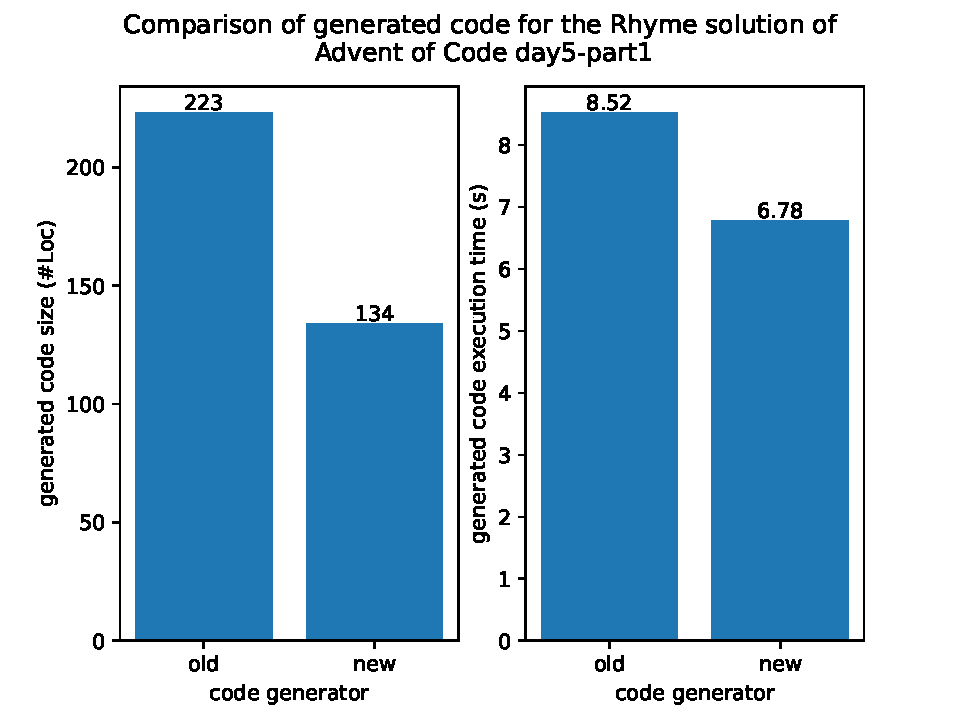
\includegraphics[scale=0.57]{figures/evaluation.pdf}
      \caption{Old vs New code generator}
      \label{evaluationpic}
  \end{figure}
As shown in Figure \ref{evaluationpic}, the JavaScript code that the old code generator generates is 223 lines while the new code generator only generates 134 lines. This is a $39.9\%$ reduction in the code size. The new code generator manages to merge more statements' loops together, therefore reducing the code size. When executing on the puzzle inputs from Advent of Code, the execution time reduces by $21.6\%$.\par

In conclusion, compared with the old code generator, our new code generator generates more efficient code by aggressively performing loop fusion at code generation time.

\section{Conclusion}\label{conclusion}
\iffalse
In this paper, we present an efficient code generation algorithm for loop-free, branch-free Rhyme IR. We present the constraints and dependencies that the code generator must follow in order to guarantee the correctness of generated code for Rhyme IR. We also present a heuristic guided loop scheduling algorithm that can achieve loop fusion at code generation time.
\fi
In this paper, we present an efficient code generation algorithm for loop-free, branch-free Rhyme IR. We present the constraints and dependencies that the code generator must follow to guarantee the correctness of the generated code for Rhyme IR. We also present a heuristic-guided loop scheduling algorithm that can achieve loop fusion at code generation time.
%\newpage
\bibliographystyle{acm}
\bibliography{paper}
\end{document}
\endinput
